\subsection{Home Assistant}
% TODO info o HA

% https://www.home-assistant.io/docs/glossary/

% jinja2 templates

% TODO verze HA, se kterou pracuji

MQTT adaptér \shellcmd{mqtt_bridge.py} popisovaný v předchozím textu
umožňuje snadnou integraci s tímto systémem. Platforma \texttt{mqtt} nabízí
v prostředí Home Assistant možnost vytvářet entity z celé řady domén~--
například \HAdomain{sensor}, \HAdomain{binary_sensor}, \HAdomain{light},
\HAdomain{switch} a další.

Příkladem funkce budíku, kterou lze do tohoto systému snadno integrovat, je
ovládání světla \uv{lamp}. To je určeno primárně pro buzení, není ale důvod,
proč by nemohlo být využíváno i pro jiné účely. Protože jde o osvětlení,
využijeme typ entity
\href{https://www.home-assistant.io/integrations/light.mqtt}{MQTT Light}.
Vlastní konfigurace je triviální:
\begin{lstlisting}[language=yaml]
light:
  - platform: mqtt
    name: AlarmClock lamp
    state_topic: alarmclock/stat/lamp
    command_topic: alarmclock/cmnd/lamp
    availability_topic: alarmclock/stat/available
\end{lstlisting}
Využíváme totiž výchozích hodnot -- například \lstinline!payload_off: OFF!
a~\lstinline!payload_on: ON!. Ty se shodují se zprávami odesílanými programem
\shellcmd{mqtt_bridge.py}. \yamlkey{availability_topic} složí k detekci
nefunkčního spojení s budíkem. V takovém případě přejde entita
\HAentity{light.alarmclock_lamp} do stavu \HAstate{unavailable}.

Platforma MQTT Light umožňuje i ovládání jasu světla, čehož využíváme
u stmívatelného LED pásku \uv{ambient}. Konfigurace je o něco složitější.
\begin{lstlisting}[language=yaml]
light:
  - platform: mqtt
    schema: template
    name: AlarmClock ambient
    availability_topic: alarmclock/stat/available
    command_topic: alarmclock/cmnd/ambient
    state_topic: alarmclock/stat/ambient
    state_template: "{{ 'off' if value == '0' else 'on' }}"
    brightness_template: "{{ value }}"
    command_off_template: 0
    command_on_template: >
      
      {{ brightness }}
      
      255
      
\end{lstlisting}
Protože je LED pásek řízen pouze jasem, kde hodnota \num{255} představuje plný
jas a \num{0} představuje zhasnuté světlo, je stav entity (zapnuto / vypnuto)
z tohoto čísla. To je úlohou šablony \yamlkey{state_template}. Protože proměnná
\texttt{value} představuje textový řetězec přijatý na \yamlkey{state_topic},
porovnáváme ji s textovým řetězcem \lstinline[language=Python]!'0'!. Druhou
možností by bylo převést \texttt{value} na celočíselný datový typ filtrem
\texttt{int} a porovnávat čísla.

\yamlkey{brightness_template} určuje, jak z přijaté MQTT zprávy odvodit jas
světla jako číslo v rozsahu \numrange{0}{255}.

\yamlkey{command_off_template} určuje zprávu, která se má poslat na
\yamlkey{command_topic}, když je požadováno vypnutí světla. Protože vypnutí
provádíme nastavením jasu na \num{0}, není ani potřeba využít šablonu.

\yamlkey{command_on_template} je složitější, protože musí správně reagovat
v různých situacích:
\begin{enumerate}[nosep]
    \item Je požadováno zapnutí světla, ale není specifikován jas. V takovém
        případě není proměnná \texttt{brightness} definována a do
        \yamlkey{command_topic} se pošle hodnota \num{255}.
    \item Je požadované zapnutí světla s určitou hodnotou jasu. V takovém
        případě se v~MQTT zprávě pošle hodnota proměnné \texttt{brightness}.
\end{enumerate}

\begin{figure}[htb]
    \centering
    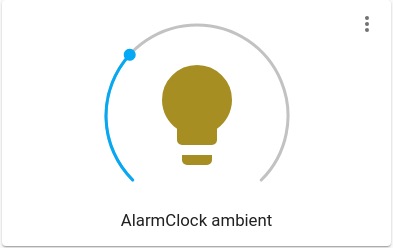
\includegraphics[width=0.3\textwidth]{homeassistant-lovelace-light}
    \caption{%
        Karta \href{https://www.home-assistant.io/lovelace/light/}{Light}
        reprezentující entitu \HAentity{light.alarmclock_ambient} v prostředí
        Lovelace systému Home Assistant
    }
    \label{fig:homeassistant lovelace light}
\end{figure}


% TODO repozitar s HA konfiguraci

\subsection{MQTT ping}  % TODO
\todo[inline]{tohle uz je outdated, bylo to nespravnym nastavenim ACL}
Kvůli chybě ve firmwaru jiného zařízení nesouvisejícího s tímto projektem
bylo odhaleno, že když dojde k zahlcení MQTT brokeru Mosquitto zprávami, dojde
k jeho selhání selhání. Zaseknutý broker nenahlásí žádné chyby, neukončí se,
takže ho \shellcmd{systemd} nemůže automaticky restartovat, nebrání klientům
v připojení, ale přestane doručovat zprávy.

Řešením problému byla oprava chyby ve firmware zmíněného zařízení. Abych
v budoucnu zabránil podobným problémům, které by mohly ovlivnit i tento
projekt, vytvořil jsem v systému Home Assistant automatizaci monitorující stav
MQTT brokeru. Automatizace zašle v případě problémů s MQTT brokerem e-mailovou
notifikaci.

Relevantní části souboru \texttt{configuration.yaml}:
\begin{lstlisting}[language=yaml]
recorder:
  # ...
  exclude:
    entities:
      - sensor.last_mqtt_ping
      # MQTT ping automation often updates last_triggered
      - automation.mqtt_ping_2
      # ...


template:
  - trigger:
      # update the sensor every minute
      - platform: time_pattern
        seconds: 3
    binary_sensor:
      - name: MQTT broker
        device_class: connectivity
        state: >-
          {{
          states("sensor.last_mqtt_ping") != "unknown" and
          as_timestamp(now()) - as_timestamp(states("sensor.last_mqtt_ping")) < 620
          }}


sensor:
  - platform: mqtt
    name: Last MQTT ping
    state_topic: mqttping


notify:
  - platform: smtp
    name: email example
    sender: homeassistant@example.com
    # recipient is only used when the service is called without a `target`
    recipient: user@example.com
    server: smtp.example.com
    port: 465
    encryption: tls
    username: !secret smtp_username
    password: !secret smtp_password

  - platform: group
    name: MQTT ping failed
    services:
      - service: email_example
        data:
          target: user@example.com
      - service: persistent_notification
\end{lstlisting}


Vlastní automatizace:
\begin{lstlisting}[language=yaml, style=numbers]
- id: '1629722205484'
  alias: MQTT ping
  description: Periodically send test message to the MQTT broker.
  trigger:
    - platform: time_pattern
      minutes: /10
    - platform: homeassistant
      event: start
    - platform: state
      entity_id: sensor.last_mqtt_ping
      to: unknown
  condition: []
  action:
    - service: mqtt.publish
      data:
        topic: mqttping
        payload_template: '{{now()}}'
  mode: single

- id: '1629722456228'
  alias: MQTT broken
  description: Notify if the MQTT broker is broken.
  trigger:
    - platform: state
      entity_id: binary_sensor.mqtt_broker
      to: 'off'
      for:
        hours: 0
        minutes: 1
        seconds: 5
  condition: []
  action:
    - service: notify.mqtt_ping_failed
      data:
        title: MQTT broker is broken
        message: |-
          MQTT pings are failing.
          Time: {{now()}}
          states("sensor.last_mqtt_ping"): {{states("sensor.last_mqtt_ping")}}
  mode: single
\end{lstlisting}


Související nastavení ACL brokeru Mosquitto:
\begin{lstlisting}
user hass
topic readwrite mqttping
\end{lstlisting}


První automatizace každých 10 minut posílá aktuální čas ve formátu ISO8601 na
topic \topic{mqttping}. Senzor \HAentity{sensor.last_mqtt_ping} zachycuje
zprávy na tomto topicu a jeho stav je shodný s payloadem přijaté zprávy.
Senzor \HAentity{binary_sensor.mqtt_broker} každou minutu ověřuje, jestli je
stav senzoru \HAentity{sensor.last_mqtt_ping} parsovaný jako čas déle starší
než \SI{620}{\second}. Pokud ano, nabývá binární senzor hodnoty \HAstate{off}.
V opačném případě nabývá hodnoty \HAstate{on}.

Druhá automatizace se spustí, pokud je stav senzoru
\HAentity{binary_sensor.mqtt_broker} \HAstate{off} déle než \SI{10}{\second},
a rozešle notifikace o zaseknutí brokeru.

